\documentclass{beamer}
\usepackage[utf8]{inputenc}
\usepackage{graphicx}
\usepackage[ngerman]{babel}
\usepackage[T1]{fontenc}

\author{Marlene Knoche}
\title{\LaTeX-Seminar}
\begin{document}

\begin{frame}

\maketitle

\end{frame}

\begin{frame}

\tableofcontents

\end{frame}

\section{Was ist \LaTeX?}

\begin{frame}{Geschichte - I}
\begin{itemize}
\item Ursprünglich wurde \TeX\; von Donald E. Knuth entwickelt
\item \LaTeX\; ist Sammlung von \TeX-Makros von Leslie Lamport 
\end{itemize}

\begin{figure}
\centering
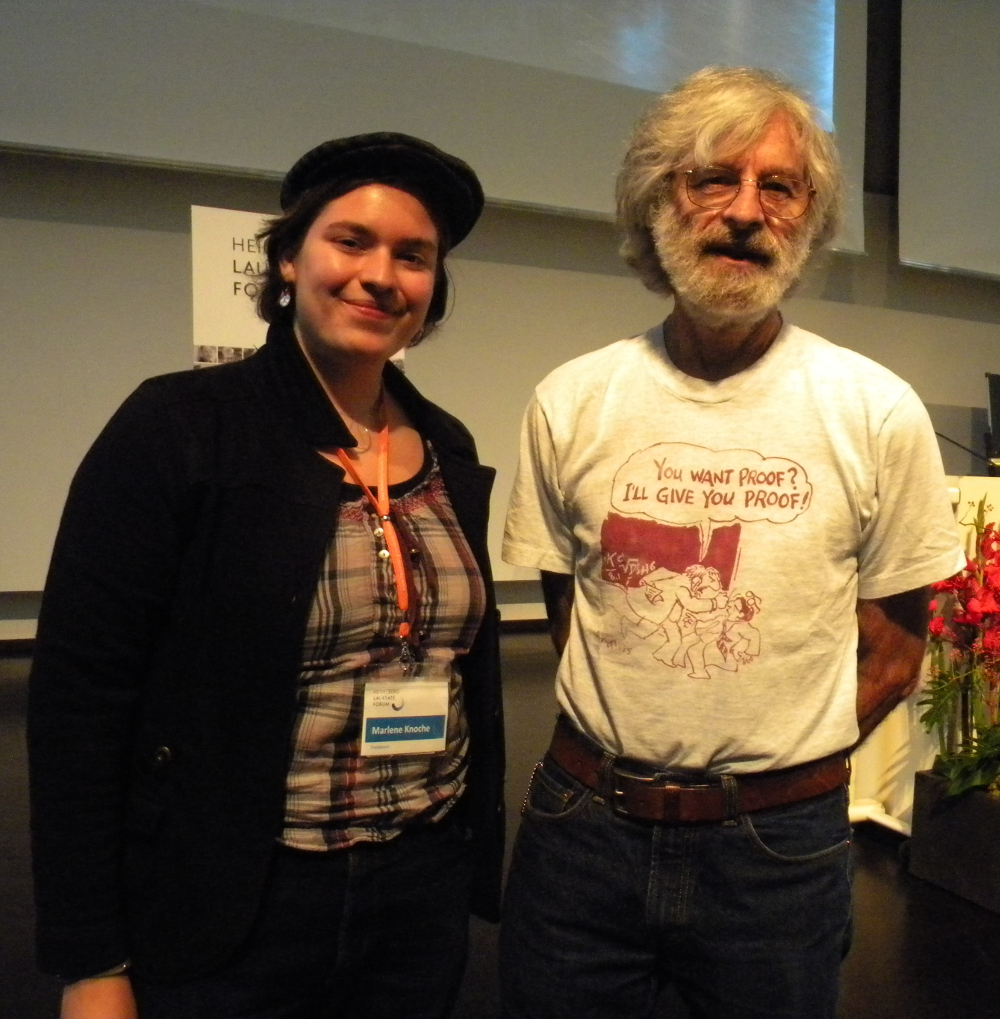
\includegraphics[scale=0.5]{pics/leslielamport.jpg}
\caption{Leslie Lamport und ich in Heidelberg beim HLF14 2014}
\end{figure}
\end{frame}

\begin{frame}{Geschichte - II}
\begin{itemize}
\item Entwicklung 1990 von Lamport eingestellt
\item Seit 1989 ist \LaTeX $2_{\varepsilon}\;$ von Frank Mittelbach, Chris Rowley und Rainer Schöpf weiter entwickelt worden
\item Seit Mitte der 1990er ist \LaTeX $2_{\varepsilon}\;$ am weitesten verbreitete Methode, \TeX\; zu nutzen
\end{itemize}
\end{frame}

\begin{frame}{WYSIWYG vs WYGIWYM}

\end{frame}

\begin{frame}{Betriebssysteme und Editoren}

\end{frame}

\section{Grundlegendes}
\begin{frame}
Hier könnte Ihr Inhalt stehen!
\end{frame}

\section{Header}
\begin{frame}
Hier könnte Ihr Inhalt stehen!
\end{frame}

\section{Body}
\begin{frame}
Hier könnte Ihr Inhalt stehen!
\end{frame}

\section{Weiterführendes}
\begin{frame}
Hier könnte Ihr Inhalt stehen!
\end{frame}

\section{Mein Template}
\begin{frame}
Hier könnte Ihr Inhalt stehen!
\end{frame}

\section{Ressourcen}
\begin{frame}
Hier könnte Ihr Inhalt stehen!
\end{frame}

\begin{frame}
\begin{center}
\huge{Fragen?}
\end{center}
\end{frame}

\end{document}